% ----------------------------------------------------
\begin{frame}
  \titlepage
\end{frame}
% ----------------------------------------------------
\note{Recordar brevemente lo visto en la clase anterior: panorama histórico del sistema internacional. Hoy: herramientas analíticas para entender la política mundial.}

% ----------------------------------------------------
\begin{frame}
\frametitle{Un marco para entender la política mundial}
\centering

\begin{itemize}
  \item ¿Por qué los Estados y otros actores toman ciertas decisiones?
  \item ¿Por qué observamos ciertos resultados y no otros?
  \item<2-> Tres conceptos clave: \textbf{intereses}, \textbf{interacciones} e \textbf{instituciones}
\end{itemize}

\end{frame}
% ----------------------------------------------------
\note{Objetivo del capítulo: presentar el marco analítico del libro (FLS). Todo el curso se apoya en estos tres conceptos. No son solo teorías: son herramientas prácticas para analizar cualquier evento internacional.}


% ====================================================
\section{Intereses}
% ====================================================

% ----------------------------------------------------
\begin{frame}
\frametitle{¿Qué son los intereses?}
\centering

\begin{itemize}
  \item Las preferencias de los actores sobre los posibles resultados de sus decisiones políticas
  \item Determinan cómo los actores ordenan los resultados: de más a menos deseado
  \item Tres grandes categorías:
  \begin{itemize}
    \item Seguridad y poder
    \item Bienestar económico
    \item Objetivos ideológicos
  \end{itemize}
\end{itemize}

\end{frame}
% ----------------------------------------------------
\note{Definición precisa: los intereses son preferencias sobre resultados. Ejemplo: EE.UU. e Irak en 2003. EE.UU. prefería (1) Irak democrático y aliado, (2) dictador pro-occidental, (3) gobierno islamista, (4) inestabilidad. Los intereses se pueden agrupar en tres categorías (seguridad, economía, ideología) que corresponden aproximadamente a las escuelas de realismo, liberalismo y constructivismo.}

% ----------------------------------------------------
\begin{frame}[plain]
  \begin{tikzpicture}[remember picture, overlay]
    \node[at = (current page.center), yshift = 0cm] (cover) {%
      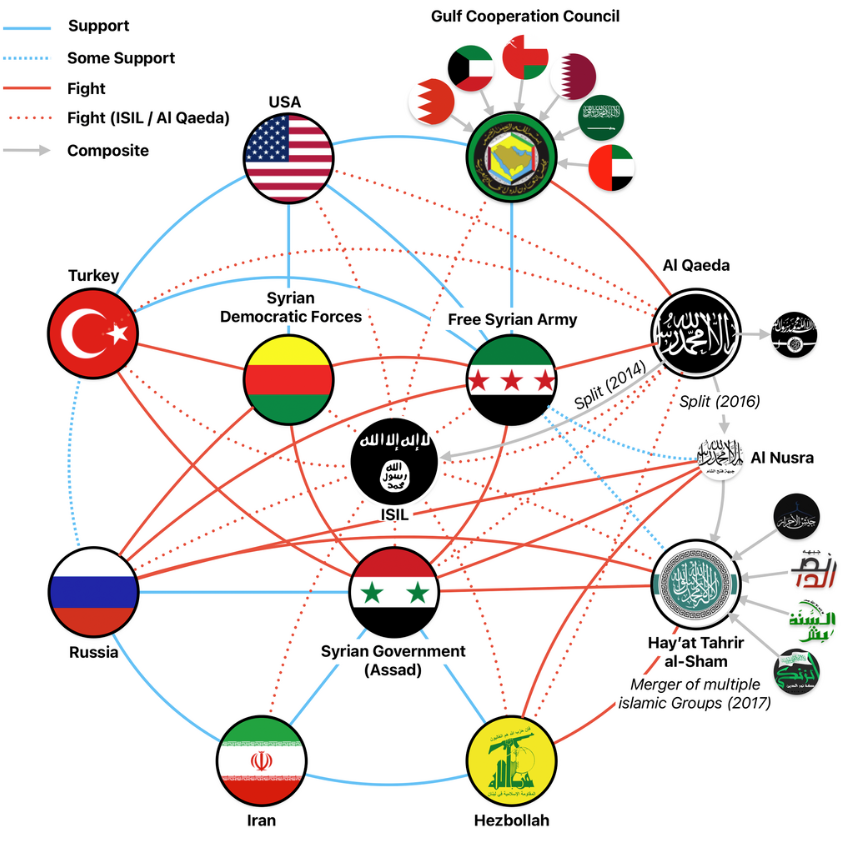
\includegraphics[keepaspectratio, height=\paperheight]{../img/actors_syriawar}};
  \end{tikzpicture}
\end{frame}
% ----------------------------------------------------
\note{Mapa de actores en la guerra de Siria. Ejemplo perfecto de la complejidad: Estados (EE.UU., Rusia, Irán, Turquía, Arabia Saudí), organizaciones internacionales (ONU), grupos armados (ISIS, rebeldes), ONGs. Cada uno con intereses distintos. Preguntar a los estudiantes: ¿qué intereses tiene cada actor?}

% ----------------------------------------------------
\begin{frame}
\frametitle{¿Quiénes son los actores?}
\centering

\footnotesize
\begin{tabular}{ll}
\textit{Tipo de actor} & \textit{Intereses típicos} \\
\hline
Estados & Seguridad, poder, riqueza \\
Políticos & Reelección, ideología \\
Empresas e industrias & Beneficios, riqueza \\
Clases / factores de producción & Bienestar material \\
Burocracias & Presupuesto, influencia \\
Organizaciones internacionales & Intereses de los miembros \\
ONGs & Derechos humanos, medio ambiente \\
\end{tabular}

\end{frame}
% ----------------------------------------------------
\note{Tabla basada en Table 2.1 del libro. Los individuos son los actores más básicos, pero es útil agruparlos. Ejemplo: Bush como jefe de Estado (interés en seguridad), como político (interés en reelección), o como individuo (ideología sobre democracia). No hay una forma ``correcta'' de definir los actores: depende del análisis.}

% ----------------------------------------------------
\begin{frame}
\frametitle{El Estado como actor}
\centering

\begin{itemize}
  \item Autoridad central capaz de crear y hacer cumplir leyes en un territorio
  \item Dos formas de entender el Estado como actor:
  \begin{itemize}
    \item Como entidad con intereses propios (\textit{interés nacional}: seguridad, poder)
    \item Como atajo para referirse a líderes que actúan en nombre del país
  \end{itemize}
\end{itemize}

\end{frame}
% ----------------------------------------------------
\note{Distinción importante. Cuando decimos ``EE.UU. amenazó a Irak'', ¿quién amenazó realmente? El presidente, los diplomáticos, los militares... El ``interés nacional'' es una simplificación útil pero puede ocultar conflictos internos. Los realistas tienden a tratar al Estado como actor unitario; otros enfoques desagregan.}

% ----------------------------------------------------
\begin{frame}
\frametitle{Soberanía y anarquía}
\centering

\begin{itemize}
  \item \textbf{Soberanía:} cada Estado tiene autoridad suprema dentro de sus fronteras
  \item \textbf{Anarquía:} no existe una autoridad central por encima de los Estados
  \item<2-> La anarquía no significa caos: significa \textit{ausencia de gobierno mundial}
\end{itemize}

\end{frame}
% ----------------------------------------------------
\note{Conceptos clave que ya vimos brevemente con Westfalia. Soberanía: nadie te dice cómo gobernar tu territorio (en teoría). Anarquía: a diferencia de dentro de un Estado, no hay policía internacional ni tribunal que pueda obligar a los Estados. Esta condición marca toda la política internacional. Ejemplo: ¿quién obliga a Rusia a cumplir el derecho internacional en Ucrania? Nadie puede, porque no hay autoridad superior.}

% % ----------------------------------------------------
% \begin{frame}
% \frametitle{Para discutir}
% \centering

% \Large ¿En qué situaciones los Estados violan la soberanía de otros Estados? ¿Cuándo es legítimo hacerlo?

% \end{frame}
% % ----------------------------------------------------


% ====================================================
\section{Interacciones}
% ====================================================

% ----------------------------------------------------
\begin{frame}
\frametitle{¿Por qué no siempre consiguen lo que quieren?}
\centering

\begin{itemize}
  \item Los resultados políticos dependen de las decisiones de \textbf{varios} actores
  \item Cada actor debe anticipar lo que harán los demás
  \item<2-> Dos tipos de interacción: \textbf{cooperación} y \textbf{negociación} (\textit{bargaining})
\end{itemize}

\end{frame}
% ----------------------------------------------------
\note{Idea central: las interacciones son estratégicas. El resultado no depende solo de lo que yo quiero, sino de lo que hacen los demás. Ejemplo: Saddam Hussein decidió resistir porque creía que Francia y Rusia bloquearían a EE.UU. en el Consejo de Seguridad. Se equivocó. Las interacciones se dividen en dos grandes tipos: cooperación (todos pueden ganar) y negociación (lo que uno gana, otro pierde).}

% ----------------------------------------------------
\begin{frame}
\frametitle{Cooperación}
\centering

\begin{itemize}
  \item Dos o más actores adoptan políticas que mejoran la situación de al menos uno \textbf{sin empeorar} la de ningún otro
  \item Juego de \textbf{suma positiva}
  \item Ejemplo: aliados cooperan para derrocar a un régimen hostil
\end{itemize}

\vspace{10pt}

\begin{tikzpicture}[scale=0.7]
  % Axes
  \draw[thick, ->] (0,0) -- (6.5,0) node[right, font=\footnotesize] {Actor A};
  \draw[thick, ->] (0,0) -- (0,5.5) node[above, font=\footnotesize] {Actor B};

  % Pareto frontier
  \draw[thick, accent] (0.5,5) -- (6,0.5);

  % Status quo
  \fill[jet] (1.5,1.5) circle (3pt) node[below right, font=\footnotesize] {$q$};

  % Shaded area (cooperation zone)
  \fill[accent!15] (1.5,1.5) -- (1.5,4.17) -- (4.87,1.5) -- cycle;

  % Points a and b on frontier
  \fill[accent] (4.87,1.5) circle (2.5pt) node[below, font=\footnotesize] {$a$};
  \fill[accent] (1.5,4.17) circle (2.5pt) node[left, font=\footnotesize] {$b$};
\end{tikzpicture}

\end{frame}
% ----------------------------------------------------
\note{Figura basada en Figure 2.1 del libro. El punto $q$ es el statu quo. El triángulo sombreado muestra todas las combinaciones que mejoran a ambos. La línea es la frontera de Pareto (máximo beneficio posible). Cooperar = moverse desde $q$ hacia la frontera. Pero ¿dónde exactamente en la frontera? Ahí entra la negociación.}

% ----------------------------------------------------
\begin{frame}
\frametitle{Negociación (\textit{bargaining})}
\centering

\begin{itemize}
  \item Los actores deben elegir resultados que benefician a uno \textbf{a costa} del otro
  \item Juego de \textbf{suma cero}: lo que uno gana, otro pierde
  \item Ejemplo: dos Estados negocian sobre un territorio
\end{itemize}

\vspace{10pt}

\begin{tikzpicture}[scale=0.7]
  % Axes
  \draw[thick, ->] (0,0) -- (6.5,0) node[right, font=\footnotesize] {Actor A};
  \draw[thick, ->] (0,0) -- (0,5.5) node[above, font=\footnotesize] {Actor B};

  % Pareto frontier
  \draw[thick, accent] (0.5,5) -- (6,0.5);

  % Arrow along frontier
  \draw[thick, accent2, <->] (1.8,4.0) -- (5.2,1.15);

  % Labels
  \node[font=\footnotesize, accent2] at (1.2,4.3) {B gana};
  \node[font=\footnotesize, accent2] at (5.8,0.85) {A gana};
\end{tikzpicture}

\end{frame}
% ----------------------------------------------------
\note{Figura basada en Figure 2.2. Cuando los actores están en la frontera de Pareto, cualquier mejora para uno implica pérdida para otro. Esto es negociación pura. Ejemplo: división de territorio, reparto de costes de una operación militar. La mayoría de las interacciones en política internacional combinan cooperación Y negociación: los actores cooperan para crear valor, pero luego negocian cómo repartirlo.}

% ----------------------------------------------------
\begin{frame}
\frametitle{Cooperación + negociación}
\centering

\begin{itemize}
  \item La mayoría de las interacciones combinan ambas
  \item Los actores cooperan para crear beneficios conjuntos...
  \item ...pero negocian sobre cómo repartirlos
\end{itemize}

\vspace{10pt}

\begin{tikzpicture}[scale=0.7]
  % Axes
  \draw[thick, ->] (0,0) -- (6.5,0) node[right, font=\footnotesize] {Actor A};
  \draw[thick, ->] (0,0) -- (0,5.5) node[above, font=\footnotesize] {Actor B};

  % Pareto frontier
  \draw[thick, accent] (0.5,5) -- (6,0.5);

  % Status quo
  \fill[jet] (1.5,1.5) circle (3pt) node[below right, font=\footnotesize] {$q$};

  % Shaded cooperation zone
  \fill[accent!15] (1.5,1.5) -- (1.5,4.17) -- (4.87,1.5) -- cycle;

  % Arrow from q to frontier (cooperation)
  \draw[thick, accent, ->] (1.5,1.5) -- (3.2,2.8);
  \node[font=\tiny, accent, rotate=40] at (2.0,2.5) {cooperación};

  % Arrow along frontier (bargaining)
  \draw[thick, accent2, <->] (1.8,4.0) -- (4.6,1.7);
  \node[font=\tiny, accent2, rotate=-32] at (3.8,3.3) {negociación};

  % Points a and b on frontier
  \fill[accent] (4.87,1.5) circle (2.5pt) node[below, font=\footnotesize] {$a$};
  \fill[accent] (1.5,4.17) circle (2.5pt) node[left, font=\footnotesize] {$b$};
\end{tikzpicture}

\end{frame}
% ----------------------------------------------------
\note{Figura clave (Figure 2.3 del libro). Primero cooperan para salir del statu quo y acercarse a la frontera. Luego negocian sobre dónde quedarse en la frontera. A prefiere estar cerca de $a$; B prefiere $b$. Si no se ponen de acuerdo sobre el reparto, la cooperación puede fracasar. Ejemplo: coalición contra Irak (2003) -- los aliados cooperan pero negocian cuánto contribuye cada uno.}

% ----------------------------------------------------
\begin{frame}
\frametitle{Tipos de cooperación}
\centering

\begin{itemize}
  \item \textbf{Coordinación:} basta con que todos hagan lo mismo
  \begin{itemize}
    \item Ejemplo: por qué lado de la carretera conducir
    \item Una vez coordinados, nadie tiene incentivos para desviarse
  \end{itemize}
  \item \textbf{Colaboración:} todos ganan cooperando, pero cada uno tiene incentivos para \textit{no} cooperar
  \begin{itemize}
    \item Ejemplo: el Dilema del Prisionero
  \end{itemize}
\end{itemize}

\end{frame}
% ----------------------------------------------------
\note{Coordinación es relativamente fácil (ejemplo: estándares internacionales de Internet, idioma de pilotos aéreos). La colaboración es el caso difícil: todos estarían mejor cooperando, pero cada uno tiene incentivos para aprovecharse. Es el problema central de la política internacional.}

% ----------------------------------------------------
\begin{frame}
\frametitle{El Dilema del Prisionero}
\centering

\vspace{-5pt}
\footnotesize

\begin{tikzpicture}[scale=0.85]
  % Headers
  \node[font=\footnotesize\bfseries] at (3.5, 3.4) {Prisionero 2};
  \node[font=\footnotesize\bfseries, rotate=90] at (-0.8, 1.5) {Prisionero 1};
  \node[font=\footnotesize] at (2.25, 2.7) {Cooperar};
  \node[font=\footnotesize] at (4.75, 2.7) {Delatar};
  \node[font=\footnotesize, rotate=90] at (0.2, 1.85) {Cooperar};
  \node[font=\footnotesize, rotate=90] at (0.2, 0.35) {Delatar};

  % Grid
  \draw[thick] (1,0) rectangle (3.5,2.4);
  \draw[thick] (3.5,0) rectangle (6,2.4);
  \draw[thick] (1,0) rectangle (3.5,1.2);
  \draw[thick] (3.5,0) rectangle (6,1.2);

  % Payoffs
  \node[font=\small, accent] at (2.25, 1.8) {1 año, 1 año};
  \node[font=\small] at (4.75, 1.8) {10 años, \textbf{libre}};
  \node[font=\small] at (2.25, 0.6) {\textbf{Libre}, 10 años};
  \node[font=\small, accent2] at (4.75, 0.6) {5 años, 5 años};
\end{tikzpicture}

\vspace{5pt}
\begin{itemize}
  \item La estrategia dominante de cada prisionero es \textbf{delatar}
  \item Resultado: ambos acaban peor que si hubieran cooperado
\end{itemize}

\end{frame}
% ----------------------------------------------------
\note{Explicar paso a paso: si mi compañero coopera, me conviene delatar (quedo libre en vez de 1 año). Si mi compañero delata, también me conviene delatar (5 años en vez de 10). Así que delatar es la estrategia dominante. Pero el resultado (5, 5) es peor para ambos que (1, 1). El dilema: la racionalidad individual lleva a un resultado colectivamente peor. Ejemplo internacional: la carrera armamentística entre EE.UU. y la URSS. Ambos habrían preferido limitar armas, pero cada uno temía que el otro siguiera armándose.}

% ----------------------------------------------------
\begin{frame}
\frametitle{Bienes públicos y acción colectiva}
\centering

\begin{itemize}
  \item \textbf{Bienes públicos:} no se puede excluir a nadie de su disfrute, y el consumo de uno no reduce la cantidad disponible
  \begin{itemize}
    \item Defensa nacional, aire limpio, erradicación de enfermedades
  \end{itemize}
  \item Problema: incentivo para ser \textbf{free rider}
  \begin{itemize}
    \item Disfrutar del bien sin contribuir a pagarlo
  \end{itemize}
  \item<2-> Dentro de un Estado, el gobierno puede obligar (impuestos)
  \item<2-> A nivel internacional... no hay quien obligue
\end{itemize}

\end{frame}
% ----------------------------------------------------
\note{Ejemplo: todos quieren que se frene el cambio climático, pero cada país prefiere que otros paguen el coste de reducir emisiones. Ejemplo histórico: algunos países se opusieron a la invasión de Irak no porque no quisieran el cambio de régimen, sino porque querían beneficiarse del resultado sin asumir los costes. El problema de acción colectiva es central en la política internacional porque no hay gobierno mundial que obligue a contribuir.}

% ----------------------------------------------------
\begin{frame}
\frametitle{¿Qué facilita la cooperación?}
\centering

\begin{itemize}
  \item \textbf{Número reducido} de actores
  \begin{itemize}
    \item Más fácil comunicarse y vigilar el cumplimiento
  \end{itemize}
  \item \textbf{Interacciones repetidas} (\textit{iteración})
  \begin{itemize}
    \item Si vamos a interactuar otra vez, el castigo futuro disuade de engañar hoy
  \end{itemize}
  \item \textbf{Información}
  \begin{itemize}
    \item Si puedo observar lo que haces, es más fácil cooperar
    \item La incertidumbre y las percepciones erróneas socavan la cooperación
  \end{itemize}
\end{itemize}

\end{frame}
% ----------------------------------------------------
\note{Tres factores clave. (1) Grupos pequeños cooperan más fácilmente (ejemplo: acuerdos bilaterales vs. acuerdos multilaterales masivos). (2) La iteración alarga la sombra del futuro; ejemplo: las trincheras de la Primera Guerra Mundial donde soldados desarrollaron un sistema de ``vivir y dejar vivir'' por la interacción repetida. (3) Información: Saddam Hussein había desmantelado sus armas pero no podía demostrarlo creíblemente; la falta de información fue clave en la guerra de Irak.}

% ----------------------------------------------------
\begin{frame}
\frametitle{¿Quién gana y quién pierde en la negociación?}
\centering

\begin{itemize}
  \item \textbf{Poder:} la capacidad de hacer que otro haga algo que no haría por sí solo
  \item El resultado de una negociación depende del \textit{reversion outcome}: ¿qué pasa si no hay acuerdo?
  \item<2-> Quien está \textbf{menos insatisfecho} con el statu quo tiene más poder de negociación
\end{itemize}

\end{frame}
% ----------------------------------------------------
\note{Definición de poder de Robert Dahl. El ``reversion outcome'' es clave: si no llegamos a un acuerdo, ¿qué pasa? Quien puede tolerar mejor la situación sin acuerdo tiene más leverage. Ejemplo: en negociaciones climáticas, EE.UU. tiene menos prisa porque está mejor preparado para afrontar el cambio climático que los países insulares. Resultado: EE.UU. puede imponer más condiciones.}

% ----------------------------------------------------
\begin{frame}
\frametitle{Herramientas de poder en la negociación}
\centering

\begin{itemize}
  \item \textbf{Coerción:} imponer costes al otro para cambiar su comportamiento
  \begin{itemize}
    \item Fuerza militar, sanciones económicas
  \end{itemize}
  \item \textbf{Opciones exteriores} (\textit{outside options}): alternativas atractivas si la negociación fracasa
  \begin{itemize}
    \item EE.UU. en 2003: podía actuar sin la ONU
  \end{itemize}
  \item \textbf{Fijación de la agenda} (\textit{agenda setting}): actuar primero para condicionar las opciones de los demás
\end{itemize}

\end{frame}
% ----------------------------------------------------
\note{Tres formas de ejercer poder. (1) Coerción: no solo capacidad material, también la disposición a asumir costes (Ho Chi Minh: ``Matarán a 10 de los nuestros y nosotros mataremos a 1 de los suyos, y al final serán ustedes los que se cansen''). (2) Outside options: EE.UU. podía ir a la guerra sin aprobación de la ONU, lo que debilitó el poder del Consejo de Seguridad. (3) Agenda setting: al llevar el tema a la ONU y luego iniciar la guerra, EE.UU. obligó a otros a reaccionar.}

% % ----------------------------------------------------
% \begin{frame}
% \frametitle{Para discutir}
% \centering

% \Large ¿Puede un actor débil tener poder sobre uno fuerte? ¿En qué circunstancias?

% \end{frame}
% % ----------------------------------------------------


% ====================================================
\section{Instituciones}
% ====================================================

% ----------------------------------------------------
\begin{frame}
\frametitle{¿Qué son las instituciones?}
\centering

\begin{itemize}
  \item Conjuntos de reglas, conocidas y compartidas, que estructuran las interacciones
  \item Pueden ser \textbf{formales} (ONU, OMC, FMI) o \textbf{informales} (normas, costumbres)
  \item<2-> En política internacional, las instituciones \textit{no pueden obligar} a los Estados a cumplir
  \item<2-> Pero facilitan la cooperación de otras formas
\end{itemize}

\end{frame}
% ----------------------------------------------------
\note{Definición clave. A nivel doméstico, el gobierno puede hacer cumplir las reglas (policía, tribunales). A nivel internacional, no hay equivalente: el sistema es anárquico. La ONU NO es un gobierno mundial. Pero eso no significa que las instituciones sean inútiles. La cooperación a nivel internacional tiene que ser auto-ejecutada (self-enforcing): los propios Estados se vigilan mutuamente.}

% ----------------------------------------------------
\begin{frame}
\frametitle{¿Cómo facilitan la cooperación?}
\centering

\begin{itemize}
  \item \textbf{Fijan estándares} de comportamiento
  \begin{itemize}
    \item Reglas claras: más fácil detectar violaciones
  \end{itemize}
  \item \textbf{Verifican el cumplimiento}
  \begin{itemize}
    \item Informes, inspecciones (ej: OIEA y armas nucleares)
  \end{itemize}
  \item \textbf{Reducen costes} de decisión conjunta
  \begin{itemize}
    \item Foros permanentes, reglas de votación establecidas
  \end{itemize}
  \item \textbf{Resuelven disputas}
  \begin{itemize}
    \item Mecanismos de arbitraje (ej: OMC)
  \end{itemize}
\end{itemize}

\end{frame}
% ----------------------------------------------------
\note{Cuatro funciones de las instituciones internacionales. (1) Estándares: la Resolución 661 de la ONU especificaba exactamente qué armas podía y no podía tener Irak. (2) Verificación: la OIEA inspecciona instalaciones nucleares en más de 70 países. (3) Costes de decisión: sin la ONU, cada negociación empezaría de cero. (4) Disputas: la OMC tiene un mecanismo de resolución de disputas que incluso países pequeños como Costa Rica han usado contra EE.UU. Ninguna de estas funciones implica ``obligar'', pero todas hacen la cooperación más probable.}

% ----------------------------------------------------
\begin{frame}
\frametitle{¿A quién benefician las instituciones?}
\centering

\begin{itemize}
  \item Las instituciones reflejan el poder de quienes las crearon
  \item Ejemplo: el \textbf{Consejo de Seguridad} de la ONU
  \begin{itemize}
    \item Cinco miembros permanentes con derecho a veto
    \item Los cinco vencedores de la Segunda Guerra Mundial
  \end{itemize}
  \item Las reglas nunca son neutrales: siempre contienen un \textbf{sesgo}
  \item<2-> Aun así, incluso los Estados desfavorecidos prefieren tener reglas a no tener ninguna
\end{itemize}

\end{frame}
% ----------------------------------------------------
\note{Las instituciones son producto de negociaciones pasadas. Quien tiene más poder cuando se crean las reglas, escribe reglas que le favorecen. Consejo de Seguridad: Francia y Rusia pudieron bloquear la guerra de Irak. FMI: EE.UU. tiene ~17\% de los votos. Pero los Estados cumplen porque: (1) la cooperación que facilitan es valiosa (ejemplo: EE.UU. cumple sentencias de la OMC para preservar el sistema de comercio libre); (2) crear instituciones nuevas es muy costoso (ejemplo: Vietnam, seis meses negociando la forma de la mesa).}

% ----------------------------------------------------
\begin{frame}
\frametitle{¿Por qué se cumplen las reglas?}
\centering

\begin{itemize}
  \item La cooperación que facilitan vale más que los costes de las reglas desfavorables
  \item Crear instituciones nuevas es \textbf{caro y lento}
  \begin{itemize}
    \item Es más fácil trabajar con las existentes, aunque sean imperfectas
  \end{itemize}
  \item<2-> Resultado: tasas de cumplimiento sorprendentemente altas en política internacional
\end{itemize}

\end{frame}
% ----------------------------------------------------
\note{Dos razones para cumplir. (1) El valor de la cooperación compensa las reglas injustas: EE.UU. cumple con la OMC no por miedo a Costa Rica, sino porque quiere preservar el sistema de libre comercio. (2) Los costes hundidos: ya se pagó el coste de crear las reglas, y crear otras nuevas requiere empezar de cero. Ejemplo: tras fracasar en la ONU con Irak, EE.UU. volvió a usar el Consejo de Seguridad para Irán en 2006. Las instituciones internacionales no son perfectas, pero las tasas de cumplimiento son más altas de lo que cabría esperar en un sistema anárquico.}


% ====================================================
\section{Teorías de las relaciones internacionales}
% ====================================================

% ----------------------------------------------------
\begin{frame}[plain]
  \begin{tikzpicture}[remember picture, overlay]
    \node[at = (current page.center), yshift = 0cm] (cover) {%
      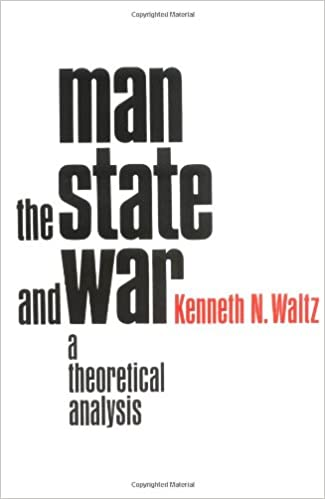
\includegraphics[keepaspectratio, height=.85\paperheight]{../img/waltz}};
  \end{tikzpicture}
\end{frame}
% ----------------------------------------------------
\note{Kenneth Waltz (1924--2013). Uno de los teóricos más influyentes de las relaciones internacionales. Su libro \textit{Man, the State, and War} (1959) organiza las explicaciones de la guerra (y de la política internacional en general) en tres niveles de análisis. Es el punto de partida para entender las grandes teorías de las RRII.}

% ----------------------------------------------------
\begin{frame}
\frametitle{Tres niveles de análisis (Waltz, 1959)}
\centering

\begin{itemize}
  \item \textbf{Primera imagen:} el individuo
  \begin{itemize}
    \item La naturaleza humana, las decisiones de los líderes
  \end{itemize}
  \item \textbf{Segunda imagen:} el Estado
  \begin{itemize}
    \item El régimen político, la política interna
  \end{itemize}
  \item \textbf{Tercera imagen:} el sistema internacional
  \begin{itemize}
    \item La estructura anárquica, la distribución de poder
  \end{itemize}
\end{itemize}

\end{frame}
% ----------------------------------------------------
\note{Waltz pregunta: ¿por qué hay guerras? Las respuestas se pueden organizar en tres niveles. (1) Primera imagen: los humanos son agresivos por naturaleza, o los líderes toman malas decisiones (ejemplo: la personalidad de Saddam Hussein). (2) Segunda imagen: los regímenes autoritarios son más belicosos, o la política interna presiona hacia la guerra (ejemplo: el lobby militar-industrial en EE.UU.). (3) Tercera imagen: la estructura del sistema internacional -- la anarquía -- obliga a los Estados a competir por su seguridad, independientemente de quién los gobierne. Waltz argumenta que la tercera imagen es la más fundamental: mientras exista anarquía, habrá conflicto.}

% ----------------------------------------------------
\begin{frame}
\frametitle{Realismo}
\centering

\begin{itemize}
  \item El sistema internacional es \textbf{anárquico}: no hay autoridad superior
  \item Los Estados son los actores principales
  \item El interés fundamental es la \textbf{seguridad} y el \textbf{poder}
  \item<2-> Los Estados desconfían unos de otros $\rightarrow$ dilema de seguridad
  \item<2-> La cooperación es difícil y frágil
\end{itemize}

\end{frame}
% ----------------------------------------------------
\note{El realismo parte de la tercera imagen de Waltz. Ideas centrales: (1) la anarquía obliga a los Estados a velar por sí mismos (self-help); (2) no importa quién gobierne -- democracias y dictaduras se comportan de forma similar bajo presión; (3) el dilema de seguridad: si yo me armo para defenderme, tú te sientes amenazado y también te armas, lo que me hace sentir más inseguro. Es un círculo vicioso. Autores clave: Tucídides, Maquiavelo, Hobbes, Morgenthau, Waltz, Mearsheimer.}

% ----------------------------------------------------
\begin{frame}
\frametitle{Liberalismo}
\centering

\begin{itemize}
  \item Hay muchos actores relevantes, no solo los Estados
  \begin{itemize}
    \item Organizaciones internacionales, empresas, ONGs, individuos
  \end{itemize}
  \item Los intereses económicos y la \textbf{interdependencia} importan tanto como la seguridad
  \item La cooperación es posible y las \textbf{instituciones} tienen un papel propio
  \item<2-> La democracia y el comercio reducen el riesgo de guerra
\end{itemize}

\end{frame}
% ----------------------------------------------------
\note{El liberalismo cuestiona al realismo en varios puntos. (1) Actores: no solo los Estados importan; las empresas, los organismos internacionales y la sociedad civil también influyen. (2) Intereses: no todo es seguridad; el comercio, la inversión y el bienestar económico son motores fundamentales. (3) Instituciones: para los liberales, las instituciones no son solo un reflejo del poder; tienen efectos independientes (facilitan cooperación, reducen incertidumbre). Idea clave: la ``paz democrática'' -- las democracias casi nunca van a la guerra entre sí. Autores: Kant, Keohane, Nye, Russett.}

% ----------------------------------------------------
\begin{frame}
\frametitle{Constructivismo}
\centering

\begin{itemize}
  \item Las \textbf{ideas}, \textbf{normas} e \textbf{identidades} dan forma a los intereses
  \item Los intereses no están dados: se construyen socialmente
  \item La anarquía no implica necesariamente conflicto
  \begin{itemize}
    \item ``La anarquía es lo que los Estados hacen de ella'' (Wendt)
  \end{itemize}
  \item<2-> Las normas internacionales pueden cambiar el comportamiento de los Estados
\end{itemize}

\end{frame}
% ----------------------------------------------------
\note{El constructivismo cuestiona las premisas de realistas y liberales. (1) Los intereses no son fijos ni ``naturales'': dependen de las ideas, la cultura y la identidad. Ejemplo: ¿por qué EE.UU. ve a las armas nucleares de Corea del Norte como una amenaza pero no a las de Francia? La diferencia está en la identidad y la relación social, no en la capacidad material. (2) Alexander Wendt: la anarquía no dicta un único comportamiento; depende de cómo los Estados se perciban mutuamente (rivales, competidores o amigos). (3) Las normas cambian: la esclavitud era aceptada, hoy es impensable. Los derechos humanos, la soberanía, la no intervención son ideas construidas históricamente. Autores: Wendt, Finnemore, Katzenstein.}

% ----------------------------------------------------
\begin{frame}
\frametitle{Las tres teorías y el marco I-I-I}
\centering

\vspace{-5pt}
\scriptsize
\begin{tabular}{l>{\raggedright\arraybackslash}p{2.2cm}>{\raggedright\arraybackslash}p{2.2cm}>{\raggedright\arraybackslash}p{2.2cm}}
 & \textbf{Realismo} & \textbf{Liberalismo} & \textbf{Constructivismo} \\
\hline
\textbf{Actores} & Estados & Estados, OO.II., empresas, ONGs & Estados y otros, definidos por su identidad \\[6pt]
\textbf{Intereses} & Seguridad, poder & Seguridad, economía, bienestar & Construidos por ideas, normas, identidad \\[6pt]
\textbf{Interacciones} & Negociación, coerción, autoayuda & Cooperación posible gracias a la interdependencia & Definidas por percepciones e identidades mutuas \\[6pt]
\textbf{Instituciones} & Reflejo del equilibrio de poder & Facilitan cooperación de forma independiente & Expresan y refuerzan normas compartidas \\
\end{tabular}

\end{frame}
% ----------------------------------------------------
\note{Tabla síntesis. Cada teoría responde de forma diferente a las preguntas del marco I-I-I. (1) Para el realismo, los Estados buscan poder y seguridad, las interacciones son competitivas, y las instituciones solo reflejan quién manda (ejemplo: el veto en el Consejo de Seguridad). (2) Para el liberalismo, hay muchos actores con intereses económicos, la cooperación es posible y las instituciones la facilitan (ejemplo: la OMC permite resolver disputas comerciales). (3) Para el constructivismo, los intereses dependen de las ideas, las interacciones dependen de cómo los actores se ven mutuamente, y las instituciones expresan normas compartidas (ejemplo: la norma de no proliferación nuclear). El libro de FLS integra elementos de las tres tradiciones sin casarse con ninguna.}

% % ----------------------------------------------------
% \begin{frame}
% \frametitle{Para discutir}
% \centering

% \Large ¿Cuál de las tres teorías explica mejor la guerra en Ucrania? ¿Y la cooperación climática?

% \end{frame}
% % ----------------------------------------------------


% ====================================================
\section{Resumen}
% ====================================================

% ----------------------------------------------------
\begin{frame}
\frametitle{Recapitulación}
\centering

\begin{itemize}
  \item \textbf{Intereses, interacciones e instituciones:} el marco analítico del curso
  \item \textbf{Tres niveles de análisis} (Waltz): individuo, Estado, sistema
  \item \textbf{Tres grandes teorías:} realismo, liberalismo, constructivismo
  \item<2-> Cada teoría ilumina aspectos diferentes de la política mundial
  \item<2-> El curso usa herramientas de las tres
\end{itemize}

\end{frame}
% ----------------------------------------------------
\note{Resumen final. Hemos visto dos cosas hoy: (1) el marco analítico I-I-I del libro, que estructura cómo pensamos sobre cualquier evento internacional; (2) las tres grandes tradiciones teóricas, que ofrecen respuestas diferentes a las preguntas fundamentales. No hay una teoría ``correcta'': cada una ilumina aspectos distintos. El curso de FLS integra las tres. La próxima semana: el problema de la guerra (capítulo 3), donde aplicaremos estos conceptos al caso más extremo de fracaso de la cooperación.}

% ----------------------------------------------------
\begin{frame}
\frametitle{}
\centering

Preguntas?

\end{frame}
% ----------------------------------------------------
\note{}
